\documentclass{article}
\usepackage{amsmath,amsthm}
\usepackage{cancel}
\usepackage{indentfirst}
\usepackage{commath}
\usepackage{pgfplots}
\begin{document}

% TODO: Pull this into a common file
% From Wikipedia, not sure where to define this yet...
\def\ci{\perp\!\!\!\perp}
\def\defeq{\buildrel\triangle\over =}
\def\E{\mathrm{E}}
\def\Var{\mathrm{Var}}
\def\Cov{\mathrm{Cov}}


\section{MLE for the Bernoulli/ binomial model}

\begin{gather}
X_i \sim Ber(\theta) \\
p(D|\theta) = \theta^{N_1}(1 - \theta)^{N_0}
\end{gather}

\begin{align*}
  \ln \left(  p(D|\theta) \right) &= \ln \left( \theta^{N_1}(1 -
                                    \theta)^{N_0} \right) \\
                                  &= \ln \left( \theta^{N-1} \right) + \ln \left( 1 - \theta
                                    \right)^{N_0} \\
                                  &= N_1 \ln \theta + N_0 \ln (1 - \theta) \\
  \od{}{\theta} \ln p(D|\theta) &= \frac{N_1}{\theta} - \frac{N_0}{1 -
                                  \theta}
\end{align*}

The log-likelihood will take a maximum when the derivative equals 0.

\begin{align*}
  0 &= \frac{N_1}{\theta} - \frac{N - N_1}{1 - \theta} \\
  0 &= N_1(1 - \theta) - \theta(N-N_1) \\
  0 &= N_1 - \theta N_1 - \theta N + \theta N_1 \\
  0 &= N_1 - \theta(N_1 + N - N_1) \\
  0 &= N_1 - \theta N \\
  \hat{\theta} &= \frac{N_1}{N}
\end{align*}
\section{Marginal likelihood for Beta-Bernoulli model}
\begin{equation}\label{chain-rule-prob}
  p(X_{1:N}) = p(x_1)p(x_2|x_1)p(x_3|x_{1:2}) ... p(x_N|x_{N-1})
\end{equation}

\begin{equation}\label{bb-post-pred}
    p(X=k|D_{1:N}) = \frac{N_k + \alpha_k}{\sum_i N_i + \alpha_i}
\end{equation}

\begin{equation}\label{gamma-def}
  (\alpha - 1)! = \Gamma(\alpha)
\end{equation}

Given $D = H,T,T,H,H \defeq 1,0,0,1,1$

\begin{gather*}
  p(X=1|\alpha) = \frac{\alpha_1}{\alpha} \\
  p(X=0|\alpha, D_1) = \frac{\alpha_0}{\alpha + 1} \\
  p(X=0|\alpha, D_{1:2}) = \frac{\alpha_0 + 1}{\alpha + 2} \\
  p(X=1|\alpha, D_{1:3}) = \frac{\alpha_0 + 1}{\alpha + 3} \\
  p(X=1|\alpha, D_{1:4}) = \frac{\alpha_0 + 2}{\alpha + 4} \\
\end{gather*}

\begin{align*}
  p(D) &= p(D_{1:5}) \\
       &= p(D_1) \cdot p(D_2|D_1) \cdot p(D_3|D_{1:2}) \cdot
         p(D_4|D_{1:3}) \cdot p(D_5|D_{1:4}) \qquad \text{by ($\ref{chain-rule-prob}$)} \\
       &= \frac{\alpha_1}{\alpha} \cdot
         \frac{\alpha_0}{\alpha + 1} \cdot \frac{\alpha_0 + 1}{\alpha + 2}
         \cdot \frac{\alpha_1 + 1}{\alpha + 3} \cdot \frac{\alpha_1 +
         2}{\alpha + 4} \qquad \text{by ($\ref{bb-post-pred}$)} \\
       &= \frac{\left[ \alpha_1 (\alpha_1 + 1) (\alpha_1 + 2) \right] \left[
         \alpha_0 (\alpha_0 + 1) \right]}
         {\alpha (\alpha + 1) (\alpha + 2) (\alpha + 3) (\alpha + 4) }
  \\
       &= \frac{\left[ (\alpha_1) ... (\alpha_1 + N_1 - 1) \right] \left[
         (\alpha_0) ... (\alpha_0 + N_0 - 1) \right]}
         {(\alpha) ... (\alpha + N - 1)} \\
       &= \frac{(\alpha_1 + N_1 - 1)!}{(\alpha_1 - 1)!} \cdot
         \frac{(\alpha_0 + N_0 - 1)!}{(\alpha_0 - 1)!} \cdot
         \frac{(\alpha - 1)!}{(\alpha + N - 1)!} \\
       &= \frac{\Gamma(\alpha_1 + N_1)}{\Gamma(\alpha_1)} \cdot \frac{\Gamma(\alpha_0
         + N_0)}{\Gamma(\alpha_0)} \cdot
         \frac{\Gamma(\alpha)}{\Gamma(\alpha + N)} \\
       &= \frac{\Gamma(\alpha_1 + N_1) \; \Gamma(\alpha_0 +
         N_0)}{\Gamma(\alpha_1) \Gamma(\alpha_0)}
         \frac{\Gamma(\alpha_0 + \alpha_1)}{\Gamma(\alpha_0 + \alpha_1 +
         N)}
\end{align*}

\section{Posterior predictive for a Beta-Binomial model}

\begin{align*}
  p(x|n,D) &= Bb(x|\alpha_0', \alpha_1', n) \\
  &= \frac{B(x + \alpha_1', n-x+\alpha_0')}{B(\alpha_1',\alpha_0')} {n
    \choose x}
\end{align*}

Given $n = 1$

\begin{align*}
  Bb(1|\alpha_0,\alpha_1,1) &= \frac{B(1 + \alpha_1,
                              \alpha_0)}{B(\alpha_1, \alpha_0)} {1
                              \choose 1} \\
                            &= \frac{\Gamma(1 + \alpha_1)
                              \Gamma(\alpha_0)}{\Gamma(\alpha_0 +
                              \alpha_1 + 1)} \cdot
                              \frac{\Gamma(\alpha_0 +
                              \alpha_1)}{\Gamma(\alpha_0)\Gamma(\alpha_1)}
  \\
                            &= \frac{\alpha_1 \Gamma(\alpha_1)
                              \Gamma(\alpha_0)}{(\alpha_0 + \alpha_1)
                              \Gamma(\alpha_0 + \alpha_1)} \cdot
                              \frac{\Gamma(\alpha_0 +
                              \alpha_1)}{\Gamma(\alpha_0)\Gamma(\alpha_1)}
  \\
                            &= \frac{\alpha_1}{\alpha_0 + \alpha_1} \\
                            &= \frac{\alpha_1}{\alpha}
\end{align*}

\section{Beta updating from censored likelihood}

Let $n$ represent the number of coin tosses. Let $X$ represent the
number of heads. Given $n = 5$ and $X < 3$, we need to compute the
posterior $p(\theta| X < 3)$ under a $B(1,1)$ prior up to
normalization constants.

\begin{align*}
  P(\theta) &= \frac{P(\theta)P(D|\theta)}{P(D)} \\
            &= \frac{P(\theta) \cdot P(X<3|\theta)}{P(X < 3)} \\
  P(\theta) &\propto P(\theta) \cdot P(X<3) \\
            &\propto B(1,1) \cdot \sum_{k=0}^2 P(k|\theta,5) \\
            &\propto \sum_{k=0}^2 {5 \choose k} \theta^k
              (1-\theta)^{5-k} \\
\end{align*}
\section{Uninformative prior for log-odds ratio}

Let $\phi = log \frac{\theta}{1-\theta}$. $p(\phi) = 1$ is equivalent
to $p(\phi) = k$, where $k$ is a constant and $0 < k < 1$.

\begin{gather*}
  \int_\phi p(\phi) d\phi = \int_\phi k d\phi = 1 \\
  d\phi = \frac{d\phi}{d\theta} d\theta \\
  \frac{d\phi}{d\theta} = \frac{d}{d\theta} \left( ln \frac{\theta}{1 - \theta} \right) \\
  = \frac{d}{d\theta} \left( \ln \theta - \ln (1 - \theta) \right) \\
  = \frac{1}{\theta} - \frac{1}{1 - \theta} \cdot -1 \\
  = \frac{1}{\theta} + \frac{1}{1 - \theta} \\
  \int_\phi k d\phi = \int_\theta k (\frac{1}{\theta} + \frac{1}{1 -
    \theta}) d\theta \\
  1 = k \int_\theta \theta^{-1} (1 - \theta)^{-1} d\theta
\end{gather*}

We recognize the final integral as the normalization constant for a
$Beta(\theta|0,0)$ distribution.

\section{MLE for the Poisson distribution}
\begin{gather*}
  P(X=k|\lambda) = e^{-\lambda}\frac{\lambda^{k}}{k!} \quad \text{for
  } k \in \left\{ 0,1,2... \right\} \\
\end{gather*}

\begin{align*}
  p(x|\lambda) &= e^{-\lambda} \cdot \frac{\lambda^{x_1}}{x_1!} \cdot
  e^{-\lambda} \cdot \frac{\lambda^{x_2}}{x_2!} \cdot ... \\
               &= \prod_{i=1}^N e^{-lambda} \cdot
                 \frac{lambda^{x_i}}{x_i!} \\
\end{align*}

Now we take the log-likelihood and find its maximum.

\begin{align*}
  \ell(\lambda) &= \ln p(x|lambda) \\
                &= \ln \left( \prod_{i=1}^N \frac{e^{-\lambda}\lambda^{x_i}}{x_i!}
                  \right) \\
                &= \ln \left( \frac{e^{-\lambda}\lambda^{x_1}}{x_1!} \cdot
                  \frac{e^{-\lambda}\lambda^{x_2}}{x_2!} \right) ... \\
                &= \sum_{i=1}^N \ln \left(
                  \frac{e^{-\lambda}\lambda^{x_i}}{x_i!} \right) \\
                &= \sum_{i=1}^N \ln (e^{-\lambda} \lambda^{x_i}) - \ln(x_i!) \\
                &= \sum_{i=1}^N \ln (e^{-\lambda}) + \ln (\lambda^{x_i}) - \ln
                  (x_i!) \\
                &= \sum_{i=1}^N -\lambda + x_i \ln \lambda - \ln
                  \left( x_i! \right) \\
                &= -N\lambda + \left( \ln \lambda \right) \sum_{i=1}^N {x_i} -
                  \sum_{i=1}^N \ln \left( x_i! \right) \\
\end{align*}
\begin{align*}
  \ell'(\lambda) &= \frac{1}{\lambda} \sum_{i=1}^N {x_i} - N = 0 \\
  \frac{\sum_{i=1}^N {x_i}}{\lambda} &= N \\
  \lambda_{MLE} &= \frac{\sum_{i=1}^N x_i}{N}
\end{align*}

\section{Bayesian analysis of the Poisson distribution}
\subsection{a.}

\begin{align*}
  p(\lambda|D) &= \frac{p(D|\lambda)p(\lambda)}{p(D)} \\
               &\propto p(D|\lambda)p(\lambda) \\
               &= \frac{e^{-N\lambda} \cdot \lambda^{\sum_{i=1}^N
                 x_i}}{\prod_{i=1}^N x_i!} \cdot \frac{\lambda^{a-1}
                 e^{-\lambda b}}{k} \\
               &\propto e^{-N\lambda - \lambda b} \cdot
                 \lambda^{a - 1 + \sum_{i=1}^N x_i} \\
               &= e^{-\lambda (N + b)} \cdot \lambda^{ \left[ a +
                 \sum_{i=1}^N x_i \right] - 1} \\
               &= Ga(\lambda | a + \sum_{i=1}^N x_i, N + b)
\end{align*}
\subsection{b.}

\begin{gather*}
  \frac{a + \sum_{i=1}^N x_i}{N + b} as a \to 0, b \to 0 \\
  = \frac{\sum_{i=1}^N x_i}{N} \\
  = \lambda_{MLE}
\end{gather*}

\section{MLE for the uniform distribution}

\subsection{a.}

\begin{align*}
  p(D|a) &= \prod_{i=1}^N p(x) \\
         &= \left( \frac{1}{2a} \right)^N I(x_1,x_2,...,x_N \in [-a,a]) \\
         &= \left\{ \begin{array}{ll}
                     \left( \frac{1}{2a} \right)^N & \mbox{if $-a \le x_i \le a, \forall i$} \\
                     0 & \mbox{otherwise} \end{array} \right. \\
\end{align*}

Now we take the derivative of the log-likelihood.

\begin{align*}
  \ell(a) &= \ln \left( \frac{1}{2a} \right)^N \\
          &= \ln 1 - \ln (2a)^N \\
          &= -N \ln (2a) \\
  \ell'(a) &= -N \frac{1}{2a} \cdot 2 \\
          &= -\frac{N}{a}
\end{align*}


\begin{figure}[h]
  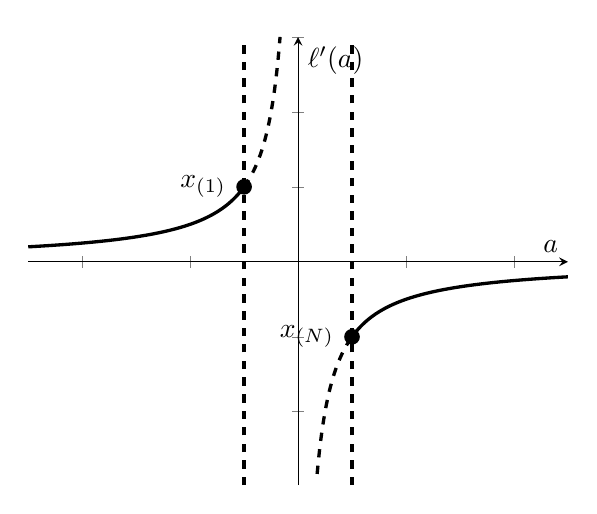
\begin{tikzpicture}
    \begin{axis}[
      samples=100,
      domain=-5:5,
      axis x line=middle,
      axis y line=middle,
      restrict y to domain=-3:3,
      xlabel=$a$,
      ylabel=$\ell'(a)$,
      xticklabels={,,},
      yticklabels={,,}]
      \addplot[
      very thick,
      dashed,
      domain=-1:1
      ] plot(\x, {-1/\x});
      \addplot[
      very thick,
      domain=-5:-1
      ] plot(\x, {-1/\x});
      \addplot[
      very thick,
      domain=1:5
      ] plot(\x, {-1/\x});
      \addplot[
      very thick,
      dashed
      ] plot(-1, \x);
      \addplot[
      very thick,
      dashed
      ] plot(1, \x);
      \node[label={180:{$x_{(1)}$}}, circle, fill, inner sep=2pt] at
      (axis cs:-1,1) {};
      \node[label={180:{$x_{(N)}$}}, circle, fill, inner sep=2pt] at
      (axis cs:1,-1) {};
    \end{axis}
  \end{tikzpicture}
\end{figure}

For $a < 0$, the likelihood is increasing, so it will be maximized
where $a = x_{(1)}$, assuming that $|x_{(1)}| \ge |x_{(N)}|$.
Similarly, for $a > 0$, the likelihood is decreasing, so it is
maximized where $a = x_{(n)}$, assuming that
$|x_{(N)}| \ge |x_{(1)}|$. This function is only defined when
$\max_i |x_i| \le a$. This means that $\ell$ is maximized at
$a = \max( |x_{(1)}|, |x_{(n)}| )$.
\end{document}
